
\section{Class Introduction}
\subsection{Outline}

\begin{frame}
  \centering
  {\huge
    Week 1 -- Part 1: Class Introduction
  }
\end{frame}

\begin{frame}
  \frametitle{Outline}
  \begin{enumerate}
    \item Class Summary
    \item What are programming Challenges?
    \item Initial Example
    \item Class Program
    \item Lecturer Introduction
    \item Extra: ICPC
  \end{enumerate}
\end{frame}

\subsection{Class Summary}
\begin{frame}{Part I: Class Summary}
  \begin{itemize}
    \item In this class, you will \structure{practice your algorithm skills by writing many programs};
    \bigskip

    \item \structure{Key Idea:} Solve challenges with programs
    \begin{itemize}
      \item Read the problem and choose the right algorithm;
      \item Choose the implementation and data structure;
      \item Run the program and check the correct result;
    \end{itemize}
    \medskip

    \item In the 1st and 2nd year, we learn the \structure{theory} of many algorithm. In this lecture, we learn the \structure{practice} of these algorithms.
  \end{itemize}
\end{frame}

\begin{frame}{Algorithms: Theory x Implementation}
  \begin{exampleblock}{}
  It is very different to implement an algorithm in the classroom, and to implement an algorithm to solve a problem:
  \end{exampleblock}
  \begin{itemize}
    \item \structure{Data Structure}: You need to implement the function to read the input and store it in a data structure;
    \item \structure{Special Cases}: Special cases in the input can cause bugs or make the problem more complex;
    \item \structure{Large Input}: If the input is very large, the implementation
    needs to be efficient, or the program will run forever;
    \item \structure{Debugging}: It can be hard to debug if the input is very hard, you need to learn how to make a \structure{test input};
  \end{itemize}
\end{frame}

\begin{frame}{Automated Judging}
  \begin{exampleblock}{}
  In this lecture we use {\bf Automated Judges (AJ)} to check the correctness of your programming assignments.
  \end{exampleblock}

  \begin{itemize}
    \item An AJ is a website that receives code from users, automatically compile it, and check its output against an expected output;
    \item AtCoder, Aizu Online Judge, Topcoder, UVA Online Judge;
    \item You can submit your code many times;
    \begin{itemize}
      \item But you don't receive debug information: you have to debug by yourself.
    \end{itemize}
    \item Grading is automatic and instantaneous;
  \end{itemize}
  \bigskip

  \begin{exampleblock}{}
  Every lecture, you have 8 programming assignments, and you have to complete a minimum of 2.
  \end{exampleblock}
\end{frame}

\begin{frame}{What this class expects of you}
  \begin{exampleblock}{Estimated classwork:}
    \begin{itemize}
      \item You need basic programming knowledge in C++ or Java;
      \medskip

      \item Complete 2-4 program assignments per week;
      \begin{itemize}
        \item (Atcoder difficulty: 300 to 500)
        \item Average of 4 hours per week
      \end{itemize}
      \medskip

      \item First assignments are easy, but later assignments are hard
      \begin{itemize}
        \item Spend a lot of time debugging and improving code;
      \end{itemize}
      \medskip

      \item No final exam: only assignments!
    \end{itemize}
  \end{exampleblock}
  \hfill Hint: Do your homework early!
\end{frame}

\subsection{What are Programming Challenges?}
\begin{frame}{Part II: What is a Programming Challenge?}
  A "Programming Challenge" is a problem where you write a program to find the solution. Think of it as a {\bf programming puzzle}:

  \begin{block}{Simple Example}
    You want to hold dancing classes. You receive a list of possible dates and
    times from all your friends (ex: Fri: 14-16). Find a set of class times
    which put most of your friends together. Don't forget to make pairs!
  \end{block}
  \bigskip

  \begin{itemize}
    \item Usually Programming challenges have a "story";
    \item Usually there is a maximum running time, so you must choose the
      most efficient algorithm;
    \item Sometimes there are special input cases;
    \item In general, you can solve the challenge with a small program (<~200 lines);
  \end{itemize}
\end{frame}


\begin{frame}{Programming Challenges in the world}
  \begin{itemize}
    \item {\bf School Competitions}: Programming contests started as a way for schools to compete early in 1980s. ICPC - University
    \bigskip

    \item {\bf Self Improvement}: After 2000, many people use online Automated Judges to improve their programming skills and compete against each other (TopCoder, HackerRank, AtCoder, etc);
    \bigskip

    \item {\bf Company Recruitment}: More recently, several companies (including Google, Facebook, etc) have started using programming challenges to test the technical knowledge of their candidates.
  \end{itemize}
\end{frame}

\subsection{Example}
\begin{frame}{A challenge example: The 3n+1 problem}
  \begin{columns}
    \column{0.6\textwidth}
      What can we expect from a programming challenge?
      \begin{itemize}
        \item Description;
        \item Input and Output format;
        \item Input and Output examples;
      \end{itemize}
      \bigskip

      Let's show how we would solve this problem (we will see more details
      later in the class).
    \column{0.4\textwidth}
    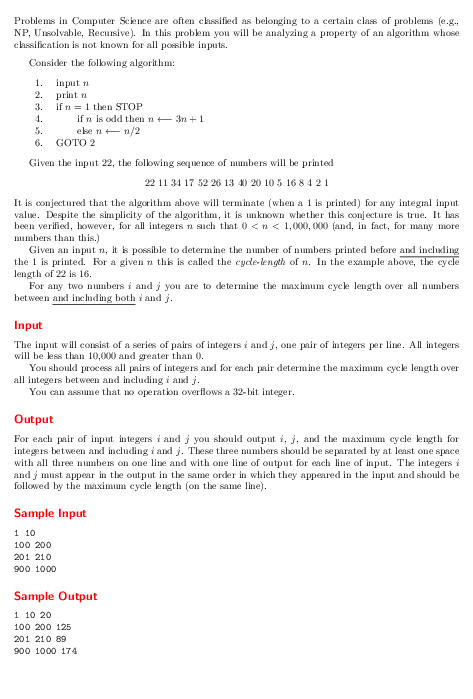
\includegraphics[width=1\textwidth]{img/3n_problem}
  \end{columns}
\end{frame}

\begin{frame}{A challenge example: The 3n+1 problem}{Solving the problem}
  \begin{columns}
    \column{0.6\textwidth}
    This problem requires that we calculate the longest sequence generated
    from the following algorithm:
      \begin{enumerate}
        \item if $n = 1$ then STOP
        \item if $n$ is odd, then $n = 3n + 1$
        \item else $n = n/2$
        \item GOTO 1
      \end{enumerate}
    \medskip

    For example, from 1 to 4:
    \begin{itemize}
      \item 1: 1 END
      \item 2: 2 1 END
      \item 3: 3 10 5 16 8 4 2 1 END
      \item 4: 4 2 1 END
    \end{itemize}
    Maximum {\bf Cycle length} is 8 (for n = 3)
    \column{0.4\textwidth}
    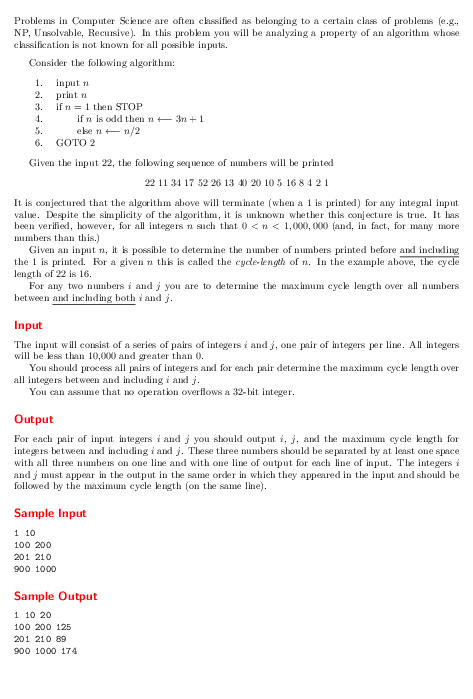
\includegraphics[width=1\textwidth]{img/3n_problem}
  \end{columns}
\end{frame}

\begin{frame}[fragile]{A challenge example: The 3n+1 problem}{A simple solution}
{\smaller
\begin{verbatim}
int main() {
  int min = 1;
  int max = 10;
  int maxcycle = 0;
  for (int i = min; i <= max; i++) {
    int cycle = 1;
    int n = i;
    while (n != 1) {
      if (n % 2 == 0) { n = n / 2; }
      else { n = n*3 + 1; }
      cycle++;
    }
    if (cycle > maxcycle) maxcycle = cycle;
  }
  cout << min << " " << max << " " << maxcycle << "\n";
  return 0;
}
\end{verbatim}}
\end{frame}

\begin{frame}{A challenge example: The 3n+1 problem}{Simple solutions, simple
  problems}
The solution proposed in the last slide has some problems. One problem is that
it can be very slow! Consider the following situation:
\bigskip

Let the input be 1 10:
\begin{itemize}
  \item 1: 1 END
  \item 2: 2 1 END
  ...
  \item 7: 7 22 11 34 17 52 26 13 40 20 10 5 16 8 4 2 1 END\\
  ...
  \item 9: 9 28 14 \alert{7 22 11 34 17 52 26 13 40 20 10 5 16 8 4 2 1 END}
  \item 10: \alert{10 5 16 8 4 2 1 END}
\end{itemize}
\bigskip

This simple program will repeat a lot of work. If the input is large, this
extra work will be very slow! How can we improve this?
\end{frame}

\begin{frame}{A challenge example: The 3n+1 problem}{Memoization}
  To solve this "repeated work" issue, we can use a technique called
  {\bf Memoization}.
  \medskip

  The basic idea is very simple: Every time you finish a calculation,
  store the result of this calculation in the memory. If you ever have to
  do that calculation again, load it from memory.
  \medskip

  This technique can be very useful to reduce the amount of repeated work.
  \bigskip

  In this course, we will review many techniques like this to make programs more efficient, and you will implement these techniques in the programming assignments.
\end{frame}

\subsection{Class Program}
\begin{frame}{Topics in this class}
  We will study the following topics in this semester:

  \begin{enumerate}
    \item Ad Hoc Problems
    \item Data Structures
    \item Search Problems
    \item Dynamic Programming
    \item Graphs Problems (Graph Structure)
    \item Graph Problems (Graph Search and Flow)
    \item String Manipulation
    \item Math Problems
    \item Geometry Problems
    \item Final Remix
  \end{enumerate}
\end{frame}

\begin{frame}{Class Format}
  \begin{block}{Weekly Lecture Contents}
    \begin{itemize}
      \item PDFs with information about algorithms
      \item Videos with explanation about the classes
      \item Programming assignments on "onlinejudge.org"
    \end{itemize}
  \end{block}

  \begin{exampleblock}{Evaluation}
    \begin{itemize}
      \item No final examination;
      \item Weekly programming assignments;
    \end{itemize}
  \end{exampleblock}
  \bigskip

  More details about these two points in the next section.
\end{frame}

\subsection{Lecturer Introduction}
\begin{frame}
  \frametitle{About the Lecturer}
  \begin{columns}
    \column{0.4\textwidth}
    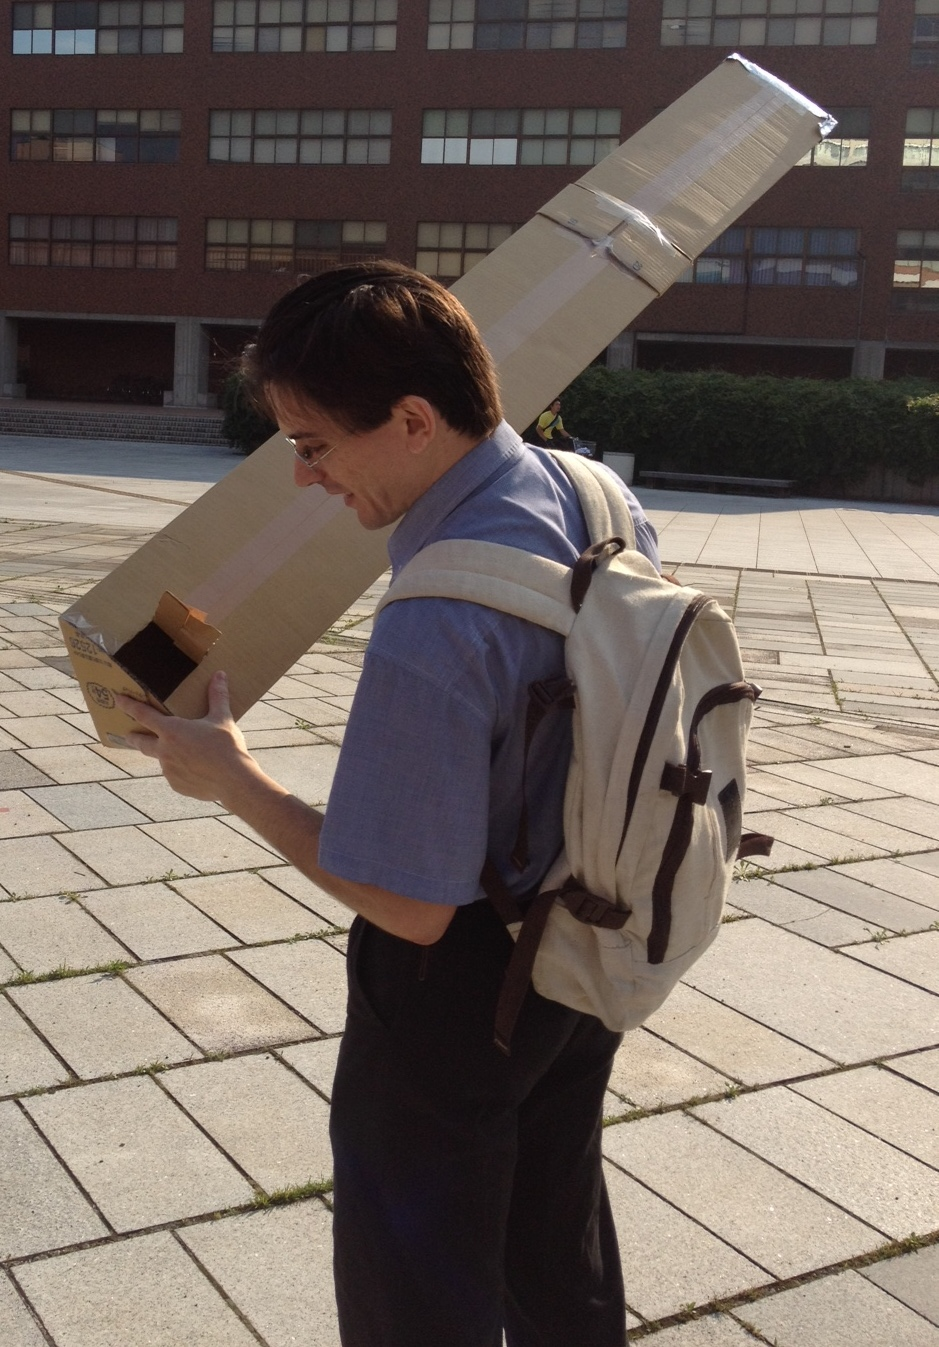
\includegraphics[width=1\textwidth]{../img/pinhole}
    \column{0.6\textwidth}
    {\small
    \begin{itemize}
      \item \structure{Name:} Claus Aranha;
      \item \structure{Country:} Brazil;
      \item \structure{Research Topics:}
      \begin{itemize}
        \item Evolutionary Algorithms;
        \item Artificial Life;
      \end{itemize}
      \item \structure{Hobbies:}
      \begin{itemize}
        \item Game Programming;
        \item Astronomy;
      \end{itemize}
        \medskip

      \item \structure{webpage:}\\ {\smaller \url{http://conclave.cs.tsukuba.ac.jp}}
    \end{itemize}
    }
  \end{columns}
\end{frame}

\subsection{ICPC}
\begin{frame}{Extra: Join the Tsukuba ICPC Team!}{What is ICPC?}
  \hfill 
\includegraphics[width=0.4\textwidth]{img/icpclogo}\\
  If you like these contests, and want an extra challenge, please consider
  joining the Tsukuba ICPC team!
  \bigskip

  ICPC (International Collegiate Programming Contest) is the largest and
  most traditional programming competition between universities.
  \bigskip

  More than 50.000 students from all over the world participate in this
  competition every year.
  \bigskip

  Contest Website: \url{https://icpc.baylor.edu/}
\end{frame}

\begin{frame}{Extra: Join the Tsukuba ICPC Team!}{Program and see the world!}
  \hfill 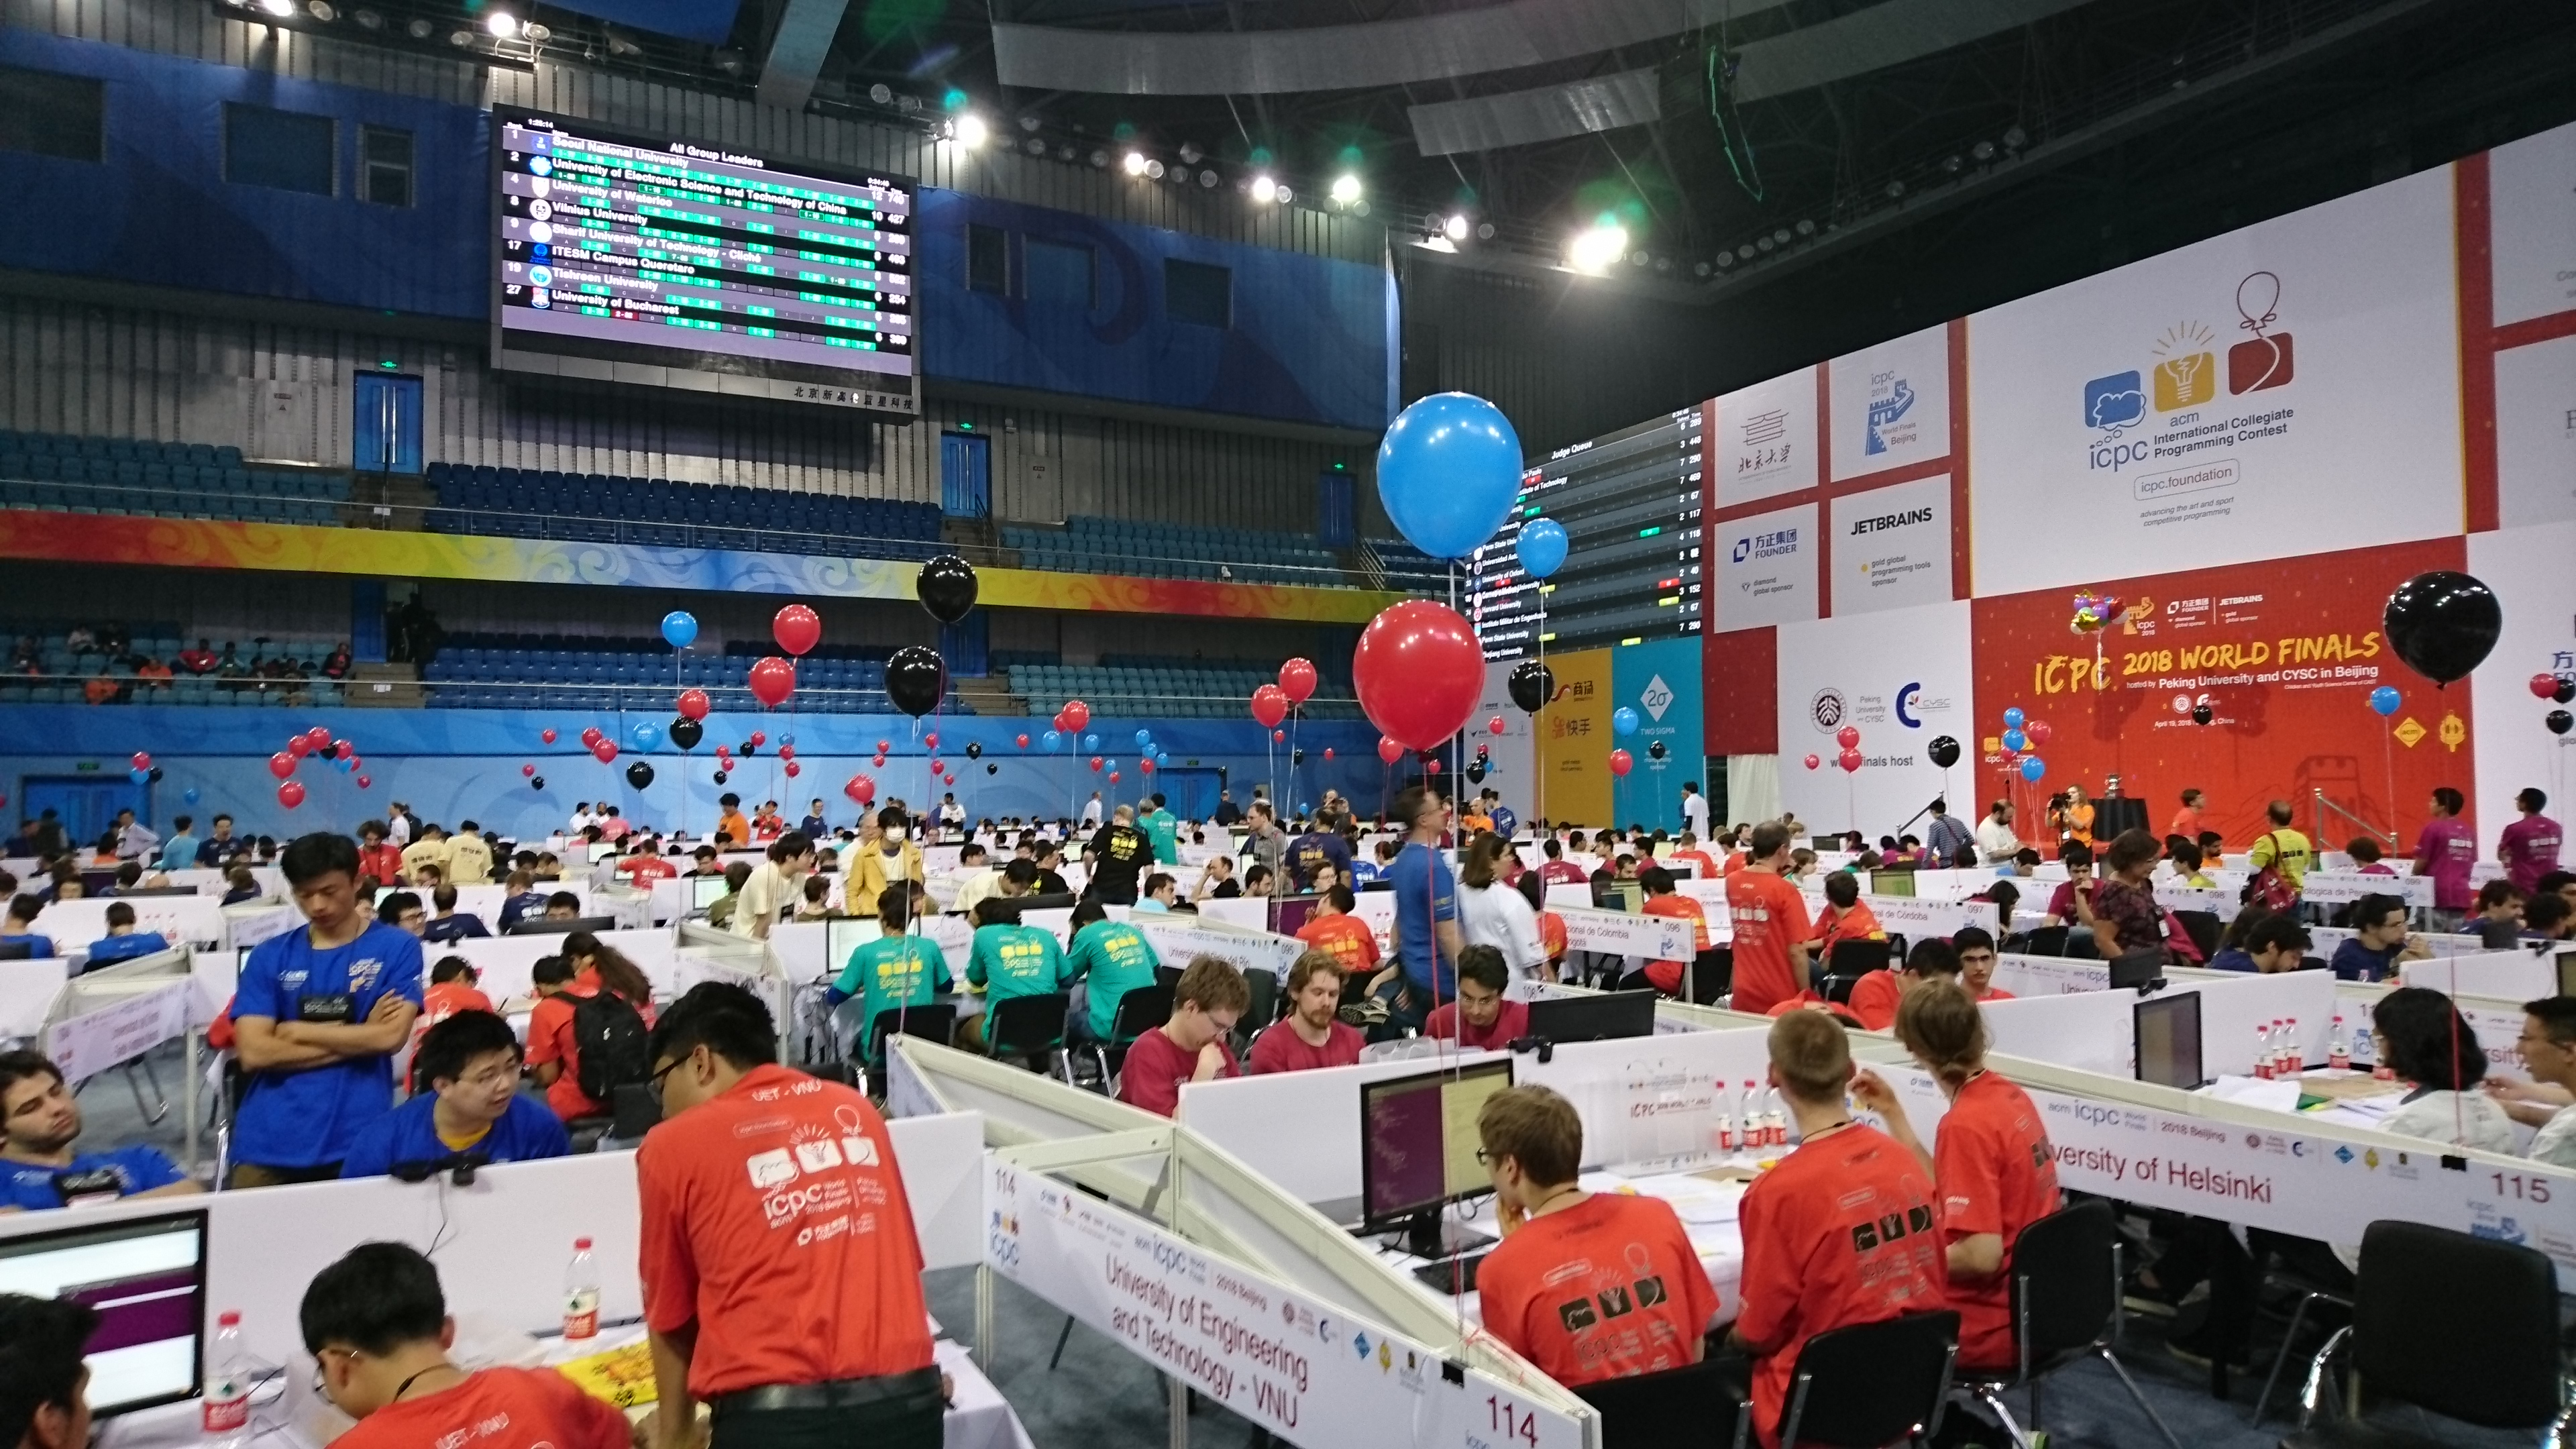
\includegraphics[width=0.4\textwidth]{img/icpc_image1}
  \begin{itemize}
    \item \alert{Requirements}: Team of 3 students, any course;
    \medskip

    \item \alert{Schedule:}
    \begin{itemize}
      \item National Preliminary Competition in July
      \item Japanese Regional Competition in October
      \item Asian Semi-final in December
      \item World Final April next year
    \end{itemize}
      (\alert{Dates may change this year because of nCov-19})
    \medskip
    \item Contact me if you're interested!
  \end{itemize}
\end{frame}



%%%%%%%%%%%%%%%%%%%%%%%%%%%%%%%%%%%%%%%%%%%%%%%%%%%%%%%%%%%%%%%%%%%%%%%%%%%%
